\documentclass[hidelinks]{article}

%%%%%%%%%%%%%%%%%%%%%%%%%%%%%%%%%%%%%%%%%%%%%%%%%%%%%%%%%%%%%%%
% START CUSTOM INCLUDES & DEFINITIONS
%%%%%%%%%%%%%%%%%%%%%%%%%%%%%%%%%%%%%%%%%%%%%%%%%%%%%%%%%%%%%%%
\usepackage{amsmath,amssymb,amsfonts,amsthm}
%\usepackage{parskip} %noident everywhere
\usepackage{mathtools}
\usepackage{subcaption}
\usepackage{overpic}
\usepackage{mymath}
\usepackage{nth}
\usepackage{caption}
\usepackage{todonotes}
\usepackage{fullpage}
\usepackage{arydshln} % dashed line in array
\usepackage{MnSymbol} % anti-diag dots
%\usepackage{showlabels} % show equation and figure labels
\usepackage{subcaption}
\usepackage{varwidth, tikz}
\usetikzlibrary{shapes, arrows, shapes.misc, arrows.meta, positioning, matrix, calc, fit, fadings, patterns}
\usetikzlibrary{calc,patterns,decorations.pathmorphing,decorations.markings,arrows, arrows.meta}
\usepackage[export]{adjustbox}
\usepackage{placeins}
%\setlength{\parindent}{0pt} 
\usepackage{tabto}

\newtheorem{lemma}{Lemma}
\newtheorem{definition}{Definition}
\newtheorem{theorem}{Theorem}
\newtheorem{corollary}{Corollary}
\newtheorem{proposition}{Proposition}
\newtheorem{assumption}{Assumption}
\newtheorem{remark}{Remark}

%%%%%%%%%%%%%%%%%%%%%%%%%%%%%%%%%%%%%%%%%%%%%%%%%%%%%%%%%%%%%%%
%%% ALG STUFF
%%%%%%%%%%%%%%%%%%%%%%%%%%%%%%%%%%%%%%%%%%%%%%%%%%%%%%%%%%%%%%%
\usepackage{algorithm}
\usepackage{algorithmic}
\newcommand{\algorithmicbreak}{\textbf{break}}
\newcommand{\Break}{\State \algorithmicbreak}
\renewcommand{\algorithmicrequire}{\textbf{Input:}}
\renewcommand{\algorithmicensure}{\textbf{Output:}}
\makeatletter
\newcommand{\algrule}[1][.2pt]{{\color{black!10!white}{\par\vskip.1\baselineskip\hrule height #1\par\vskip.1\baselineskip}}}
\makeatother
%\usepackage[linesnumbered,ruled,vlined]{algorithm2e}
%%%%%%%%%%%%%%%%%%%%%%%%%%%%%%%%%%%%%%%%%%%%%%%%%%%%%%%%%%%%%%%
% END CUSTOM INCLUDES & DEFINITIONS
%%%%%%%%%%%%%%%%%%%%%%%%%%%%%%%%%%%%%%%%%%%%%%%%%%%%%%%%%%%%%%%

\pdfobjcompresslevel=0

\title{Dykstra's Alternating Projection for Polyhedral Sets}
\author{Claudio Vestini and Idris Kempf}
\begin{document}
\maketitle

\section{Introduction}

Euclidean projections are ubiquitous in engineering, optimisation, and machine learning, playing a central role in many algorithms for solving problems constrained by complex sets. Mathematically, a projection of a point $x^\circ\in\R^n$ onto a closed convex set $\mathcal{H}\subset \R^p$ is defined as the point $x^\star\eqdef \mathcal{P}_{\mathcal{H}}(x)$ that minimises the Euclidean distance between $x^\circ$ and any point in $\mathcal{H}$:
\begin{align}\label{eq:projection}
\mathcal{P}_{\mathcal{H}}(x)\eqdef \argmin_{x\in\mathcal{H}}\twonorm{x-x^\circ}.
\end{align}
By the convexity of the set $\mathcal{C}$, problem~\eqref{eq:projection} admits a unique solution~\cite[Ch.\ 3.2]{BAUSCHKEBOOK}. Here, we assume that $\mathcal{H}$ is a convex polyhedral set that can be represented as
\begin{align}\label{eq:polyhedron}
\mathcal{H}\eqdef\set{x\in\R^p}{A x \leq c},
\end{align}
where $\inR{A}{n}{p}$ and $c\in\R^n$. Each row of $\mathcal{H}$ corresponds to a half-space $\mathcal{H}_i$,
\begin{align}\label{eq:sets_i}
\mathcal{H}_i\eqdef\set{x\in\R^p}{\trans{x}f_i \leq c_i},
\end{align}
where $f_i$, $\twonorm{f_i}=1$, is the normal vector of the plane $H_i$,
\begin{align}\label{eq:sets_i2}
H_i\eqdef\set{x\in\R^p}{\trans{x}f_i = c_i}.
\end{align}
The polyhedral set~\eqref{eq:polyhedron} can also be represented as the intersection of the half-spaces $\mathcal{H}_i$, i.e.\ $\mathcal{H}=\bigcap_{i=0}^{n-1}\mathcal{H}_i$. In many engineering applications, constraint sets can be approximated using~\eqref{eq:polyhedron}.

While for some sets the solution of~\eqref{eq:polyhedron} can be obtained explicitly and in closed form, no closed-form solution is known for an arbitrary polyhedral sets. In these cases, the solution can be obtained using a solver for constrained quadratic programs. To solve~\eqref{eq:projection}, most solvers require introducing an additional variable $z\eqdef Ax$ that is projected onto the set $\set{z\in\R^n}{z \leq c}$, for which an explicit solution exists. However, for large $n$, this variable augmentation can reduce the computational efficiency, in particular when the projection is part of a larger iterative algorithm.

As an alternative to variable augmentation, problem~\eqref{eq:projection} can be solved using \emph{Dykstra's Alternating Projection Algorithm}~\cite{DYKSTRA}. Dykstra's algorithm, first published in 1983, extends von Neumann's \emph{Method of Alternating Projections} (MAP)~\cite{NEUMANN}, which is designed to find a point lying in the intersection of $n$ closed convex sets by cyclically projecting onto each individual set. While von Neumann's algorithm identifies \emph{some} point in the intersection, Dykstra's algorithm determines the Euclidean projection~\eqref{eq:projection}. Both algorithms circumvent the potentially complex projection $\mathcal{P}_\mathcal{H}$ by iteratively applying the (known) projections $\mathcal{P}_{\mathcal{H}_0},\dots,\mathcal{P}_{\mathcal{H}_{n-1}}$. 

Although Dykstra's algorithm is proven to eventually converge to the projection, it has shown to be prone to \emph{stalling}~\cite{DYKSTRASTALLING} for certain sets, including polyhedral sets like~\eqref{eq:polyhedron}. In such cases, the iterates of Dykstra's method remain unchanged for a number of iterations. The duration of the stalling period cannot be determined \emph{a priori}, and depending on the starting point, can be arbitrary long. This phenomenon hinders the application of Dykstra's method in practice. Additionally, the algorithm \emph{cannot} be run for a fixed number of iterations with a guarantee that the output will be closer to the projection than the initial point -- a guarantee typically required when embedding Dykstra's method in iterative schemes, such as gradient methods~\cite{FGMPROJECTION}.

\section{Dykstra's Alternating Projection}\label{sec: dykstra}

Given $n$ convex sets $\mathcal{H}_0,\dots,\mathcal{H}_{n-1}$, Dykstra's alternating projection algorithm~\cite{DYKSTRAPERKINS} finds the orthogonal projection $x^\star$ of $x^\circ$ onto $\mathcal{H}\eqdef{\bigcap}_{i=0}^{n-1} \mathcal{H}_i$ by generating a series of iterates \{$x_{m}$\} using the scheme
\begin{subequations}\label{eq:dykstra}
\begin{align}
x_{m+1}&=\mathcal{P}_{\mathcal{H}_{[m]}}\left(x_{m}+e_{m-n}\right),\label{eq:dykstra:proj}\\
e_m&=e_{m-n}+x_{m}-x_{m+1}\label{eq:dykstra:error},
\end{align}
\end{subequations}
where $[m]\eqdef m \, \text{mod} \, n$, $x_0=x$, $\mathcal{P}_{[m]}\eqdef\mathcal{P}_{\mathcal{H}_{[m]}}$, and the auxiliary variables $e_m$ are initialised as
\begin{align}\label{eq:initial error}
&e_{-n} = e_{-(n-1)} = ... = e_{-1} = 0.
\end{align}

Note that von Neumann's MAP can be obtained from~\eqref{eq:dykstra} by setting $e_m \equiv 0\quad\forall m$. The Boyle-Dykstra theorem~\cite{DYKSTRA} implies that $\lim_{m\rightarrow\infty}\anynorm{x_m-\mathcal{P}_\mathcal{H}(x)}=0$. For a finite number of iterations, there is no guarantee that $x_m\in\mathcal{H}$ nor that $x_m\neq x$. 

\subsection{The Polyhedral Case}

For polyhedral sets~\eqref{eq:sets_i}, the projection step~\eqref{eq:dykstra:proj} can be simplified to
\begin{align}\label{eq:dykstra:proj:poly}
x_{m+1}=
\begin{cases}
x_{m}+e_{m-n} & \text{if } x_{m}+e_{m-n}\in\mathcal{H}_{[m]}\\
x_{m}+e_{m-n} - \left((x_{m}+e_{m-n})^\Tr f_{[m]} - c_{[m]}\right) f_{[m]} & \text{if } x_{m}+e_{m-n}\not\in\mathcal{H}_{[m]}
\end{cases},
\end{align}
and the update for the auxiliary vector to
\begin{align}\label{eq:dykstra:error:poly}
e_m=
\begin{cases}
0 & \text{if } x_{m}+e_{m-n}\in\mathcal{H}_{[m]},\\
\left((x_{m}+e_{m-n})^\Tr f_{[m]} - c_{[m]}\right) f_{[m]} & \text{if } x_{m}+e_{m-n}\not\in\mathcal{H}_{[m]},
\end{cases}.
\end{align}
The auxiliary vector $e_m$ is either $0$ or parallel to $f_{[m]}$, so that it can be represented as $e_m = k_m f_{[m]}$ with $k_m=\text{dist}_{\mathcal{H}_{[m]}}(x_{m-1}+e_{m-n})$, further simplifying~\eqref{eq:dykstra:error:poly} to
\begin{align}\label{eq:km}
k_m = k_{m-n} + x_m^\Tr f_{[m]} - c_{[m]}.
\end{align}

The convergence of Dykstra's method has been analysed in~\cite{DYKSTRAPOLY2,DYKSTRAPOLY,DYKSTRAPERKINS} for polyhedral sets. The proof is based on partitioning the sets into inactive ($x^\star\not\in H_i$) and active sets ($x^\star\in H_i$), i.e.\
\begin{align}
&A=\set{i\in\lbrace 0,\dots,n-1\rbrace}{x_\infty\in H_i},
&B=\lbrace 0,\dots,n-1\rbrace\backslash A,
\end{align}
where $x_\infty=\lim_{m\rightarrow\infty}x_m$. It can be shown that there exists a number $N_1$ such that whenever
\begin{align}
[m]\in B,\quad m\geq N_1\quad\Rightarrow\quad x_m=x_{m-1},\quad e_m=0,
\end{align}
i.e. the half-spaces that become ``inactive'' remain inactive. Furthermore, there exists $N_2\geq N_1$ such that whenever $n\geq N_2$, it holds that
\begin{align}\label{eq:dykstra:error:poly}
\twonorm{x_{m+n}-x_\infty}\leq\alpha_{[m]}\twonorm{x_m-x_\infty},
\end{align}
where $0\leq\alpha_{[m]}<1$ are numbers related to angles between half-spaces. The number $N_2$ describes the iteration from which on the algorithm has determined the inactive half-spaces. Finally, it is shown that the algorithm satisfies the following inequality:
\begin{theorem}[Deutsch and Hundal~\cite{DYKSTRAPOLY}]
There exist constants $0\leq c < 1$ and $\rho > 0$ such that
\begin{align*}
\anynorm{x_m -x_\infty} \leq \rho c^m.
\end{align*}
\end{theorem}
The factor $c$ can be estimated from the smallest $\alpha_{[m]}$, which is characterized by the angle between certain subspaces (subspaces formed by the ``active'' halfspaces). The factor $\alpha_{[m]}$ can be upper-bounded by considering the ``worst'' angles in the polyhedron. The constant $\rho$, however, depends on a number $N_3\geq N_2$ and on $x$. It is unclear how to obtain that constant $\rho$. In fact, the authors of~\cite{DYKSTRAPERKINS} and~\cite{XUPOLY} emphasize that $\rho$ cannot be computed in advance, and that the inability to compute a bound on the projection error makes the application of Dykstra's method difficult. The authors of~\cite{DYKSTRAPERKINS} proposed a combined Dysktra-conjugate-gradient method that allows for computing an upper bound on $\anynorm{x_m -x_\infty}$. The authors of~\cite{XUPOLY} proposed an alternative algorithm called \emph{successive approximate algorithm}, which promises fast convergence, conditioned on knowing a point $x\in\mathcal{H}$ in advance.

\begin{remark}[Random thoughts]
Dykstra's method could be interpreted as an autonomous non-linear discrete-time system with initial condition $x^\circ$. For $m\geq N_2$, I believe that the discrete-time system becomes \emph{linear} and could be reformulated as $x_{m+n} = G x_m + b$.
Since by the Boyle-Dykstra theorem $x_{m+n}$ necessarily converges to the projection for $n\rightarrow\infty$, the matrix $G$ must be Schur stable, so that the projection can be obtained from $x^\star = \inv{\left(I-G\right)} b$. The question is whether $N_2$ can be detected (may have been answered in the literature already).
\end{remark}

\section{Stalling}

In~\cite{DYKSTRASTALLING}, the behaviour of Dykstra's method is analysed for two sets. The authors give conditions on Dykstra's algorithm for (i) finite convergence, (ii) infinite convergence, and (iii) stalling followed by infinite convergence. A specific example is given for the case that the set is provided by the intersection of a line with a unit box in $\R^2$ ($\mathcal{H}$ is a polyhedron). It can be shown that cases (i)--(iii) depend on the starting point $x_0$, and one can determine the 3 regions shown in Figure~\ref{fig:region} that yield different convergence behaviour. Convergence case (i) is obtained when starting in the green region, case (ii) when starting in the blue region, and case (iii) when starting in the red region.

To understand the stalling effect, consider Figure~\ref{fig:stalling}, which shows the first iterations of Dykstra's algorithm with starting point in the red region. Note that the outcome of Dykstra's algorithm depends on the order of the sets $\mathcal{H}_i,\dots,\mathcal{H}_n$. In Figure~\ref{fig:stalling}, the algorithm starts by projecting onto the box and then onto the line. It can be seen that for the first 6 iterations\footnote{By one iteration we mean one cycle of $n$ projections here.}, Dykstra's algorithm returns the top left corner of the box (``stalling''). The authors also determine the exact number of iterations required to break free from the red region, and show that if the starting point is arbitrarily far to the left, the algorithm will need an arbitrarily large iteration number to break free from the red region.

% Figure demonstrating the stalling problem
\begin{figure}[h]
    \centering
    \begin{subfigure}[t]{0.49\textwidth}
        \centering
        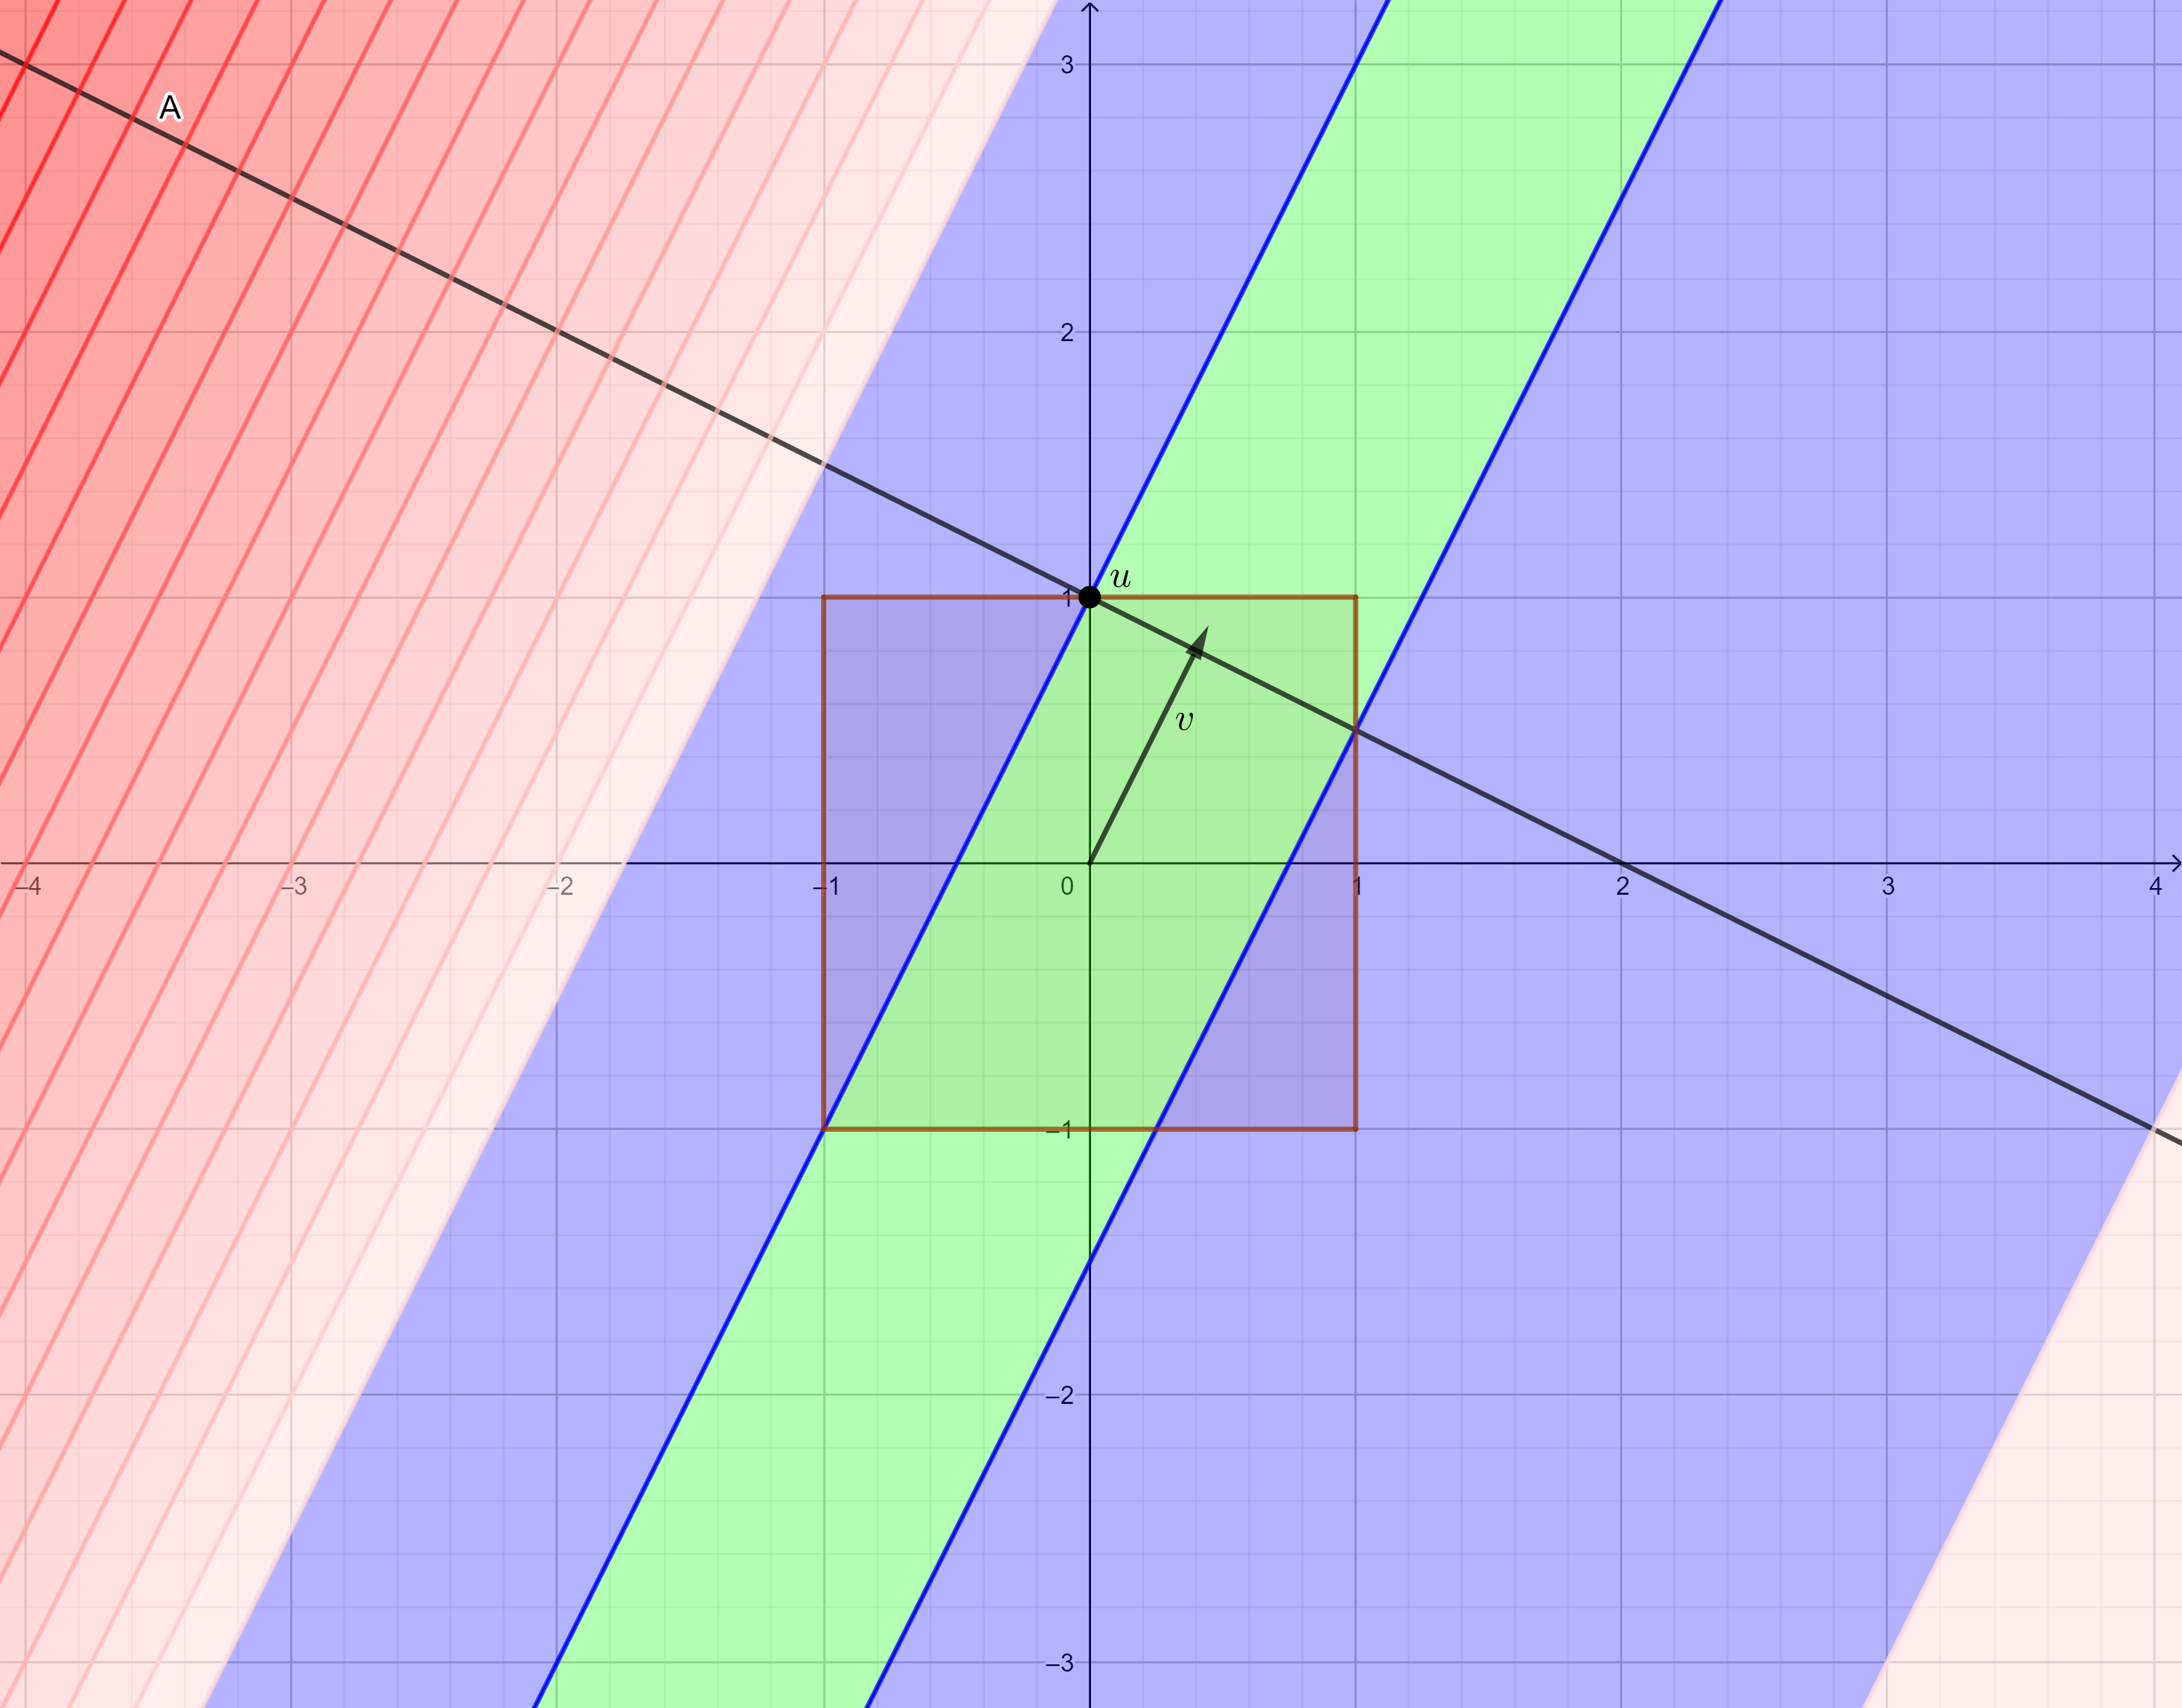
\includegraphics[width=1\textwidth]{Latex/Current Version/Figures/StallingRegionsHand.png}
        \caption{Line-box example with different regions that yield different convergence properties.}
        \label{fig:region}
    \end{subfigure}
    \hfill
    \begin{subfigure}[t]{0.49\textwidth}
        \centering
        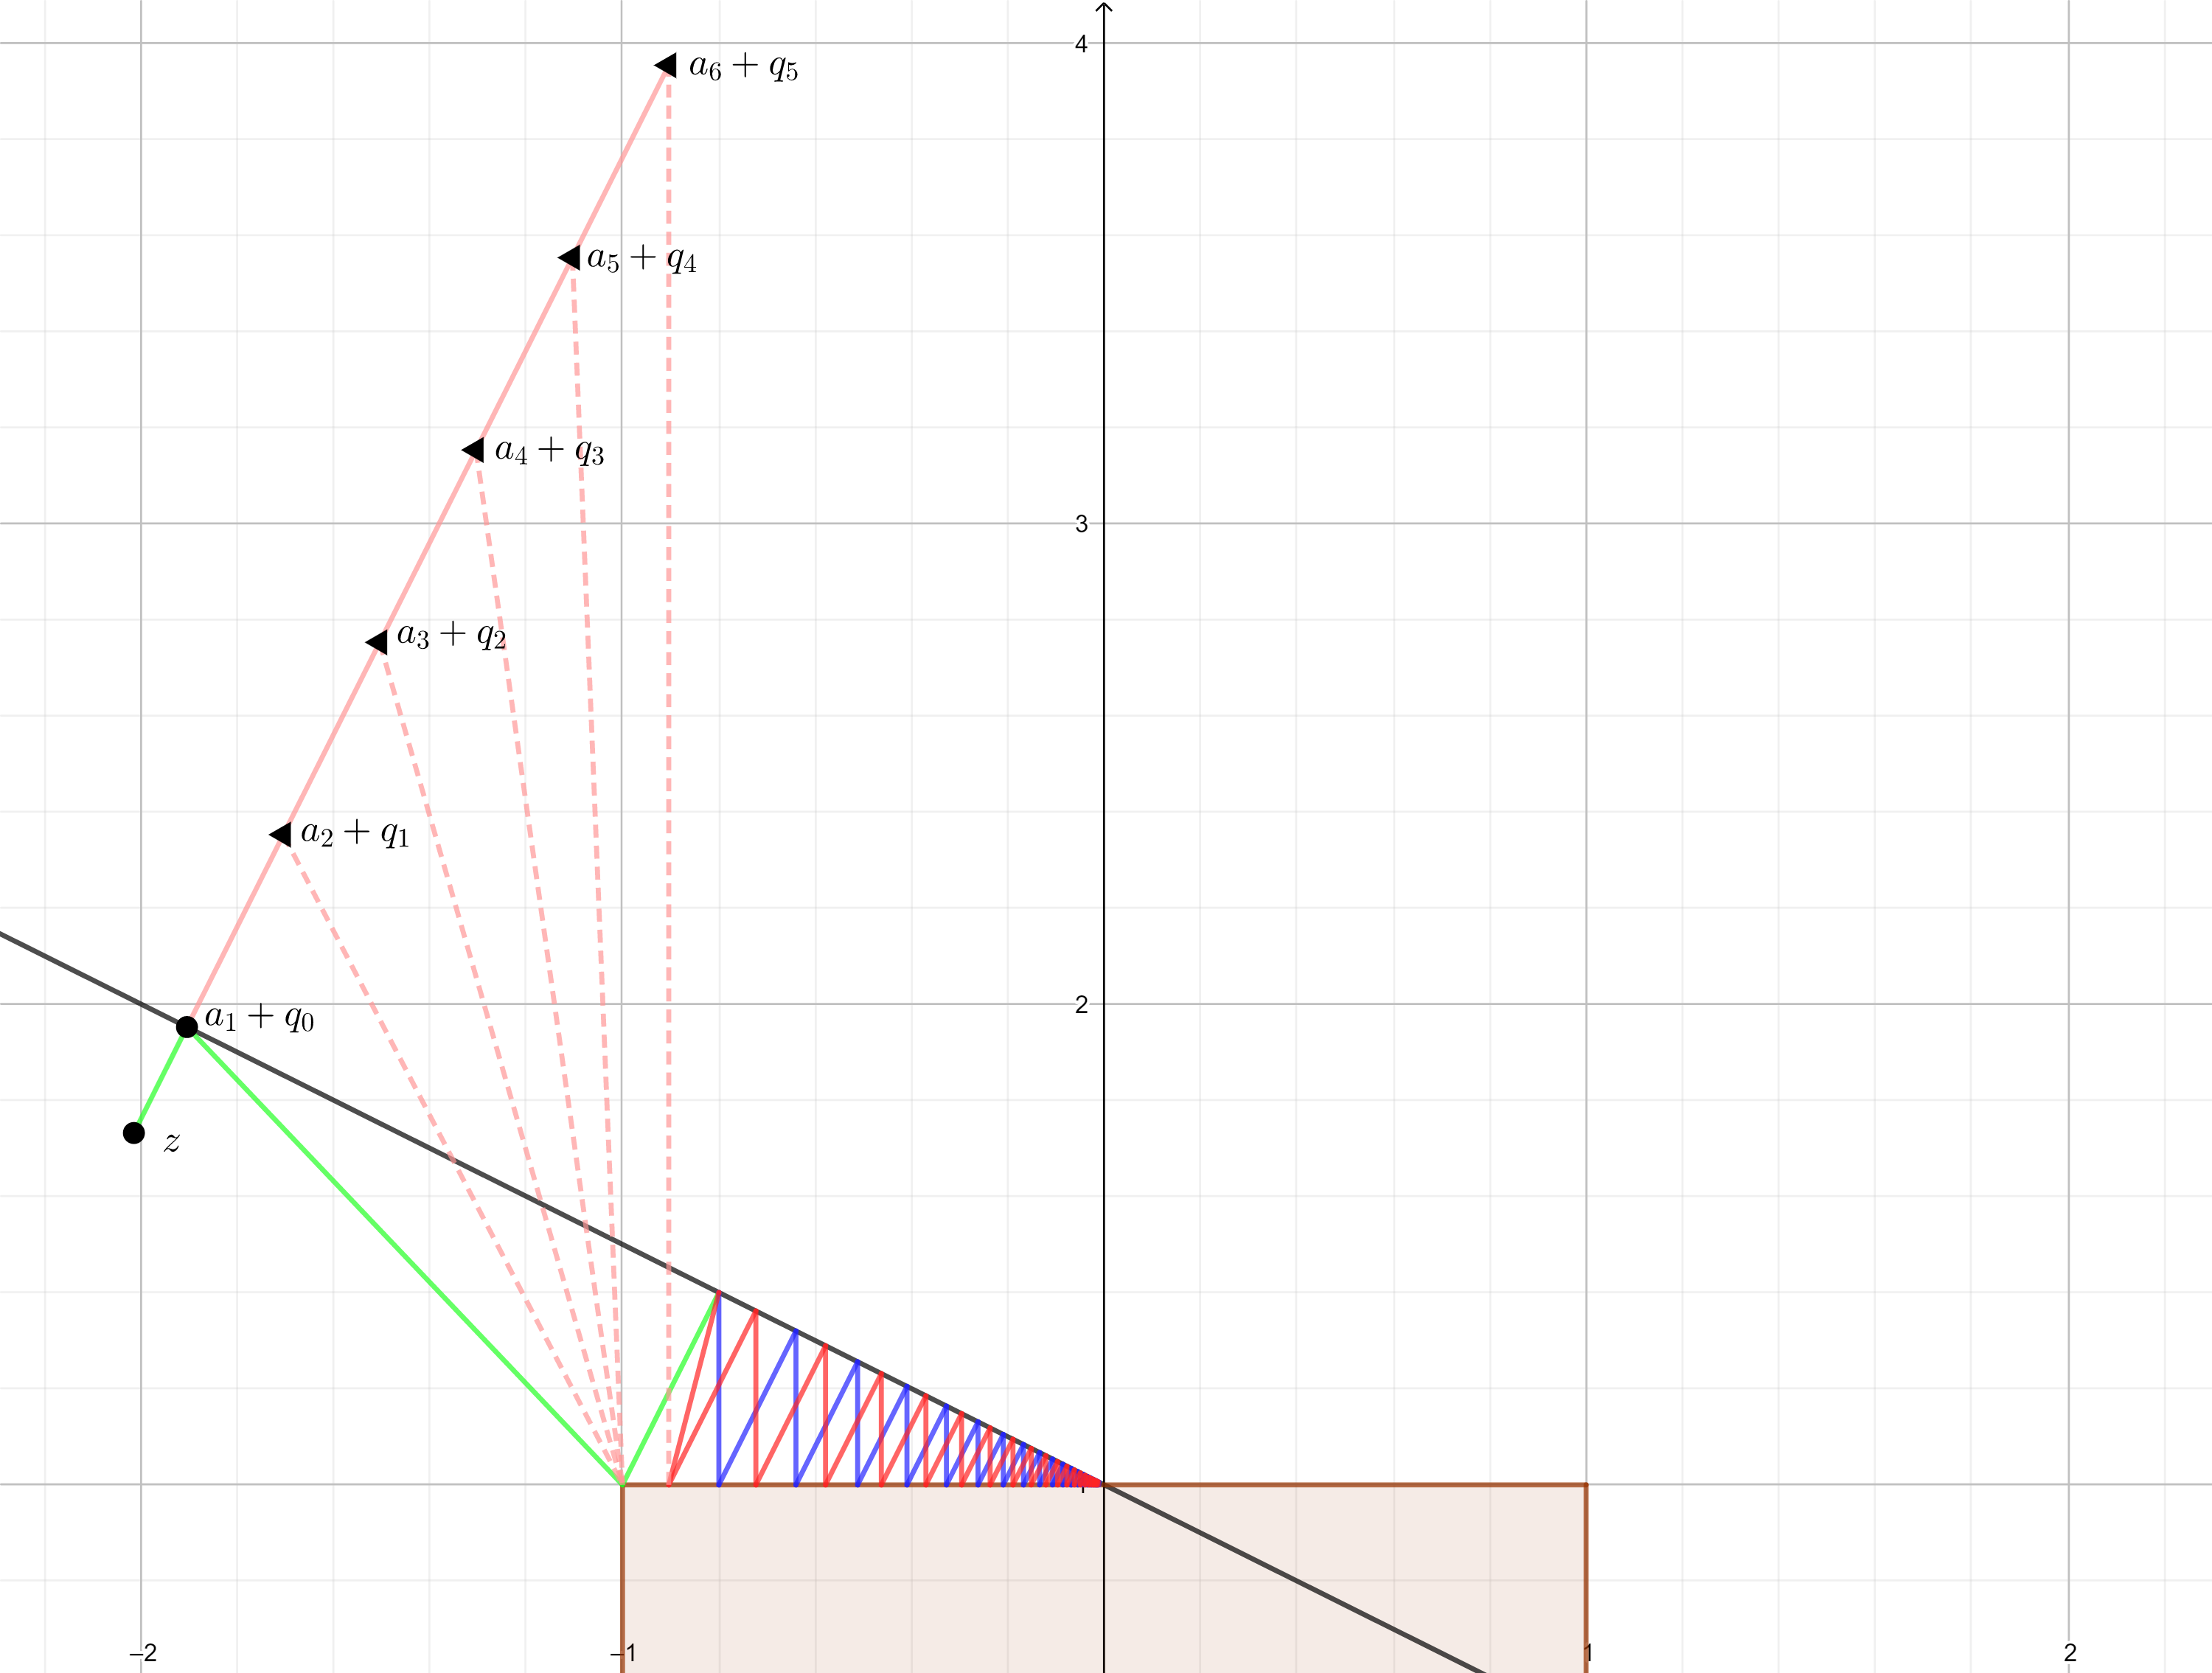
\includegraphics[width=1\textwidth]{Latex/Current Version/Figures/DifferentSequences.png}
        \caption{Stalling for the line-box example when $x_0$ is in the red region.}
        \label{fig:stalling}
    \end{subfigure}
    \caption{A demonstration of the stalling problem for a box and a line. Note how MAP applied to the same constraint sets would not result in any stalling: MAP follows the green line, and subsequently converges via the blue line path. Figure taken from~\cite{DYKSTRASTALLING}}
    \label{fig:baushkeStall}
\end{figure}

\subsection{Early Termination of Stalling}

By graphical examination of Figure~\ref{fig:baushkeStall} and formulae~\eqref{eq:dykstra}, we make the following observations:
\begin{enumerate}
\item The stalling period continues until one of the half-spaces that is active for $x^\circ$ and inactive for $x^\star$ changes from active to inactive. This is a necessary condition.
\item During stalling, it holds that $x_m\equiv x_{m-n}\quad\forall m$, so that every iteration, a constant vector $x_{m-1}-x_m$ is added to $e_m$.
\end{enumerate}

Since during stalling all $x_m$ are constant for each half-space $[m]$, the only way a half-space can become inactive is through change of the auxiliary variables $e_m$ or their length $k_m$. Moreover, increasing $k_m$ will only move $x_m+e_{m-n}$ away from the half-space, from which we follow that if a half-space is to become inactive, then the magnitude of the auxiliary variables must decrease. From~\eqref{eq:km}, $k_m$ decreases iff
\begin{align}\label{eq:exitcond}
x_m^\Tr f_{[m]} - c_{[m]} < 0.
\end{align}
Moreover, since during stalling $x_m$ is constant, there must exist at least one $m$ for which~\eqref{eq:exitcond} holds. If~\eqref{eq:exitcond} for multiple $m$, then the stalling period can be exited by making several half-spaces inactive. Suppose that stalling starts at iteration $m$ with $x_{m+i}=x_{m+n+i}$ for $i=0,\dots,n-1$, then the length of the stalling period can be computed from choosing the smallest positive integer $p_{[m+i]}$ for which
\begin{align}
k_{m+i}+p_{[m+i]}\left(x_{m+i}^\Tr f_{[m+i]} - c_{[m+i]}\right).
\end{align}
Alternatively, suppose that $\mathcal{S}\eqdef\set{i\in\lbrace 0,\dots,n-1\rbrace}{x_{m+i}^\Tr f_{[m+i]} - c_{[m+i]}<0}$, then the length of the stalling period is
\begin{align}
N_{stall}\eqdef\argmin_{i\in\mathcal{S}} \left\lfloor -k_{m+i} / \left(x_{m+i}^\Tr f_{[m+i]} - c_{[m+i]}\right)\right\rfloor.
\end{align}

Suppose that stalling is registered at iteration $m$, i.e.\ $x_{m+i}=x_{m+n+i}$ for $i=0,\dots,n-1$, then the stalling period can be skipped by applying $N_{stall}$ steps.

\section{Additional Ideas}

For the polyhedral case, Dykstra's method can be split into two phases: An first phase of length $N_2$ during which some half-spaces become inactive, and a second phase during which the algorithm iterates between active half-spaces. Note that stalling can only occur during the first phase.

For the first phase, the term $x_m^\Tr f_{[m]} - c_{[m]}$ in~\eqref{eq:km} seems to play an important role: the only way a half-space can become inactive is by obtaining a negative $x_m^\Tr f_{[m]} - c_{[m]}$. In~\cite{DYKSTRAPERKINS}, it is shown that
\begin{align}
x_{m+n} =\spanv{x_m, f_0,\dots,f_{n-1}}.
\end{align}
Moreover, by examination of~\eqref{eq:dykstra:proj:poly}, if $x_{m+n}+e_m\not\in\mathcal{H}_{[m]}$, we see that
\begin{align}
x_{m+n} =x_m + a_{[m]}f_{[m]}-\sum_{i\in \mathcal{I} \backslash [m]} a_i f_i,
\end{align}
where $a_i\geq 0$, $a_{[m]}\equiv k_m$, and $\mathcal{I}\eqdef \lbrace 0,\dots,n-1\rbrace$.

\bibliographystyle{plain}
\bibliography{master_bib_abbrev}
\end{document}